\documentclass[anonymous,12pt]{iopjournal}
\usepackage{amsmath,amssymb,amsthm,booktabs,array,microtype,graphicx,placeins}
\graphicspath{{figures/}}
\hypersetup{hidelinks,pdftitle={Material contrast bounds from finite-aperture electromagnetic scattering data},pdfauthor={},pdfsubject={Electromagnetic inverse scattering}}
\fancyhead[L]{\small\sffamily Inverse Problems\quad Research paper}
\fancyhead[R]{\small Material contrast from scattering}
\newtheorem{theorem}{Theorem}[section]
\newtheorem{proposition}[theorem]{Proposition}
\newtheorem{lemma}[theorem]{Lemma}
\newcommand{\C}{\mathbb C}\newcommand{\R}{\mathbb R}
\newcommand{\Herm}{\operatorname{Re}_{H}}\newcommand{\Imag}{\operatorname{Im}_{H}}
\newcommand{\tr}{\operatorname{tr}}\newcommand{\diag}{\operatorname{diag}}\newcommand{\Tail}{\mathcal T}
\newcommand{\rank}{\operatorname{rank}}\newcommand{\ran}{\operatorname{ran}}\newcommand{\norm}[1]{\left\|#1\right\|}
\numberwithin{equation}{section}
\setlength{\headheight}{17pt}\setlength{\emergencystretch}{1.7em}
\setcounter{topnumber}{3}\setcounter{bottomnumber}{2}
\renewcommand{\topfraction}{.92}\renewcommand{\textfraction}{.06}
\begin{document}
\noindent{\sffamily\small RESEARCH PAPER}\par\vspace{1.8ex}
\title{Material contrast bounds from finite-aperture electromagnetic scattering data}
\author{}
\begin{abstract}
Can finite-aperture scattering measurements establish that a dielectric exceeds a given contrast somewhere in the search region? We bound the distance from the measured complex fields to all responses attainable with a proposed upper limit on dielectric contrast. Completing the current quadratic leaves a matrix on illuminations. Its leading eigenvalues can be lost to negative current directions. The local material equation specifies the positive current that must accompany such a direction and retains the illumination-dependent center of the quadratic. This gives a partial compensation bound and a converse for spatially sparse sets of constitutive rows. On six lossless targets with 9,216 independent contrasts, at a cap of one and 2\% noise, no choice of up to 59 separately weighted constitutive rows can exclude the cap for the fixed current operator. For each target the data also give a positive lower bound on the norm of the physical current in the span of the thirteen negative modes. Discarding that space precludes a fit. For materials with known loss angle, dissipated power instead bounds a matrix ellipsoid of receiver fields. On a compact scatterer at two loss angles, separate multipliers for coherent illuminations exclude a cap which every common multiplier misses using the same dissipative information. The receiver ellipsoid remains too broad on the larger domain. The results identify when an array can rule out a material class before reconstruction, and when the obstruction lies in the available current bounds.
\end{abstract}
\keywords{inverse electromagnetic scattering, dielectric contrast, finite aperture, optical theorem, multiple illumination, dissipation, uncertainty bounds}

\section{Introduction}

A microwave measurement can discredit an image in two different ways. The predicted field of that image may miss the measured field. More decisively, every dielectric limited to the image's peak contrast may miss it, however the material is rearranged. The latter conclusion would tell an investigator to relax the contrast range before running another inversion. Establishing it calls for a lower bound in measured field units over all allowed distributions, including those a reconstruction method has never visited. We consider this question for nonlinear transverse-magnetic scattering from a bounded object, with finite aperture, a prescribed error radius and several illuminations.

A measured field determines only the part of the contrast current visible to the receivers. Subspace optimization and its twofold and Fourier implementations distinguish these currents in order to reconstruct an image \cite{chen,zhong,ffttsom}. Contrast-source and contraction integral equations impose the field and material relations during the iteration \cite{csi,nie,cie}. A receiver-null current may still carry power out of the measured aperture. Equally important, the currents driven by different incident fields must all give the same dielectric at each point. These requirements constrain the unmeasured currents even when the support and the image are entirely unknown. A reduction of the current space must preserve the data-dependent stationary response as well as the count of exceptional modes, a distinction that can be tested in the full array.

Conservation-based bounds in photonics have a close mathematical connection. Quadratic wave-equation constraints underlie computational limits for scattering and design \cite{angeris19,trivedi,angeris}. Global and spatially resolved power balances limit the response of a scatterer \cite{moleskyglobal,moleskylocal,kuang}, including its response to multiple excitations \cite{shim}. Absorptive response is controlled by the material factor $|\chi|^2/\Im\chi$ \cite{miller}. Our inverse question fixes a measured complex receiver matrix and allows every dielectric in a specified class. In optimizing a distance to those data, a negative quadratic form can remove only a limited number of independent eigenvalues from that particular matrix. A relaxation that averages quadratic moments can miss this pointwise rank restriction \cite{tian}. An optical equality and a sector inequality are useful on either side of the design--inverse distinction.

Finite-measurement stability and uniqueness of coefficient reconstruction require assumptions on the admissible coefficients and data \cite{alberti19,alberti21}. Monotonicity methods compare scattering operators up to finite-dimensional subspaces to localize material inhomogeneities \cite{griesmaier_harrach,griesmaier_harrach_erratum,albicker}. Here all voxel values can vary independently and the observable is a lower bound on a peak. A positive distance to a material class is compatible with poor image recovery. It also differs from enumerating roots in a small parameter model or constructing a complete set inversion \cite{everett96,vasco,sivia}, and from recovery with localized scatterers or scattered-field completion \cite{chai,levinson}.

Our analysis follows the fate of a single matrix of illumination residuals. First, the number of negative directions of a weighted current operator determines how many source eigenvalues may be lost. Enforcing the local constitutive equation restricts some of these directions and charges the illumination-dependent cost of doing so. This gives both a distance bound and an upper limit on what sparse, separately weighted constitutive rows can establish at fixed state weights. Completing just the positive square also bounds the amount of physical current in the negative modes required by any fit to the measured data. Second, a positive material loss floor restricts the same currents to an ellipsoid. Its projection onto the measured ports allows each coherent illumination to carry its own penalty. A calculation on the same data and the same material class distinguishes that choice from every common dissipative penalty. Finally, by comparing lower bounds with forward evaluations of candidate media, we distinguish failure of a relaxation from evidence that a low-contrast material actually exists.

\section{The measurement and the material hypothesis}\label{sec:model}

Take the convention $\exp(-\mathrm i\omega t)$ and a nonmagnetic dielectric invariant along the electric polarization. In the transverse plane, $j=\chi E$ obeys
\begin{equation}
 (\Delta+k^2)E=-k^2j,\qquad E=b+k^2\Phi_k*j,\qquad
 \Phi_k(x)=\tfrac{\mathrm i}{4}H_0^{(1)}(k|x|).
 \label{eq:vie}
\end{equation}
The scattered field at the receivers is the volume potential in \eqref{eq:vie}. On a grid of $n$ cells, let $B$ contain $s$ incident fields and $S$ the map from a current to $p$ receiver samples. The corresponding full-wave current, total field and data are
\begin{equation}
 E=B+GJ,\qquad J=XE,\qquad F(X)=SJ,\qquad X=\diag(\chi_1,\ldots,\chi_n).
 \label{eq:discrete}
\end{equation}
All experiments use the regular outgoing solution. Where a finite discretization could admit several states, a lower bound established for every physical pair $(X,J)$ also holds on their union. In the synthetic experiments, collocation uses the equal-area disk integral \cite{richmond,colton,chenbook}. For a square cell of width $h$, set $q=kh/\sqrt\pi$ and $c_q=\pi qJ_1(q)/2$. The off-diagonal entries are $\mathrm i c_q H_0^{(1)}(k|x_i-x_j|)$ and the self term is $\mathrm i\pi q H_1^{(1)}(q)/2-1$. A receiver outside the domain uses the off-diagonal expression. This specifies the sign, scaling and cell model of every field below.

A peak hypothesis specifies a class $\mathcal K_u$. In the lossless experiments it is the entire box $0\le\chi_i\le u$. In a fixed-loss-angle experiment it is $\chi_i=(1+\mathrm it)x_i$ with $0\le x_i\le u$, and $u$ bounds the \emph{real} contrast. Vacuum is included in both classes. The distance in measured field units is
\begin{equation}
 \delta(u;Y)=\inf_{X\in\mathcal K_u}\|F(X)-Y\|_F .\label{eq:dist}
\end{equation}
A lower endpoint above the joint error radius $r$ excludes the whole class. An upper endpoint at or below $r$, obtained from a physical medium in the class, establishes compatibility. A small lower endpoint alone leaves the question open. Material distributions enter the lower-endpoint calculations only through their measured data and the declared class.

Write $\Herm A=(A+A^*)/2$, $\Imag A=(A-A^*)/(2\mathrm i)$, and $R=\Imag G$. For real lossless contrast and diagonal weights $D_\mu\succeq0$ and $D_\lambda=D_\lambda^*$, the field obeys the two source-matrix relations
\begin{align}
 Q_r&=J^*D_\mu J-u\Herm(J^*D_\mu E)\preceq0,&
 Q_o&=\Imag(J^*D_\lambda E)=0. \label{eq:balances}
\end{align}
They follow by substituting $J=XE$. They apply to every coherent combination of the measured illuminations. At a single cell write $j,e$ for its current and total-field rows. For $a\in\ker e$ the sector inequality gives $ja=0$, hence $j=\alpha_i e$ whenever $e\ne0$. A vanishing $e$ forces $j=0$. The optical equality makes $\alpha_i$ real and the sector gives $\alpha_i\in[0,u]$. This observation explains both the value of keeping the cross-illumination terms and the information lost in spatial averaging.

For $\chi=(1+\mathrm it)x$ at fixed $t$, the disk inequality $|\chi|^2\le (1+t^2)u\,\Re\chi$ gives a legal sector. The fixed phase supplies $\Imag(J^*D E)+t\Herm(J^*D E)=0$ for real diagonal $D$. A rectangular passive range in the complex plane need not lie in this disk. The lossless optical equality is specific to the real class.

For the real box put $Z=(uD_\mu+\mathrm iD_\lambda)/2$. Expanding $\mathsf D=(SJ-Y)^*(SJ-Y)$ and adding the two physical balances gives the following pointwise minorant.
\begin{align}
 \mathsf D&\succeq Y^*Y+J^*KJ-J^*L-L^*J,&
 K&=S^*S+D_\mu-ZG-G^*Z^*,& L&=S^*Y+ZB. \label{eq:quadratic}
\end{align}
For a different material class we use only combinations of its own valid balances. The results below require \eqref{eq:quadratic}, and thus apply to those combinations as well. For nonsingular $K$ set
\begin{equation}
 J_0=K^{-1}L,\quad E_0=B+GJ_0,\quad H=Y^*Y-L^*K^{-1}L .
 \label{eq:center}
\end{equation}
$J_0$ is the stationary current of this quadratic form. It can fail the material equation at many cells. The size and orientation of those failures are observable through the known operators and $Y$.

\section{How much of the illumination response must remain?}\label{sec:bound}

For an $s\times s$ Hermitian $H$ order its eigenvalues downwards and write
$\Tail_m(H)=\sum_{j=m+1}^{s}(\lambda_j(H))_+$, with the empty sum equal to zero. If $\mathsf D\succeq0$ and $n_-(\mathsf D-H)\le m$, interlacing gives
$\lambda_i(\mathsf D)\ge\lambda_{i+m}(H)$ for $i+m\le s$ \cite{fan,tian}. Diagonalizing $H$ shows that $\Tail_m(H)$ is the sharp lower bound on $\tr\mathsf D$ given just these two restrictions. Different valid bounds on the same ordered eigenvalue can be maximized before the eigenvalues are added.

Write $K=V_+\Lambda_+ V_+^*-V_-\Lambda_- V_-^*$, with both diagonal matrices positive, and $\nu=n_-(K)$. Let $N=V_-\Lambda_-^{-1/2}$ and $P=V_+\Lambda_+^{-1/2}$. Completing the square and writing $J=J_0+NC+PU$ gives
\begin{equation}
 \mathsf D\succeq H+U^*U-C^*C . \label{eq:started}
\end{equation}
Without another restriction on the negative term, $\delta^2\ge\Tail_{\nu}(H)$. This result binds together all columns of the residual. Treating each illumination separately can spend the same $\nu$ current directions many times.

\subsection{What a current supported on the negative directions must drive}

At cell $i$ the constitutive law with real contrast $x_i$ requires
\begin{align}
 f_i(x_i)U&=d_i(x_i)-a_i(x_i)C,\qquad d_i(x)=x(E_0)_{i,:}-(J_0)_{i,:},\nonumber\\
 (a_i(x),f_i(x))&=e_i^\top(I-xG)[N,P]. \label{eq:rows}
\end{align}
where $e_i$ denotes a cell coordinate vector. For fixed $x$ and $C$, stack any rows in the form $F_+U=Z_c$. There is a solution only when $F_+F_+^\dagger Z_c=Z_c$. Among these solutions the least possible $U^*U$ in the matrix order is $Z_c^*(F_+F_+^*)^\dagger Z_c$. Indeed $U=F_+^\dagger Z_c+U_\perp$ and $F_+U_\perp=0$, so the two Gram matrices add. This is exact elimination for these rows at the specified material values. Minimizing the resulting physical outer problem over all allowable values and discarding the other rows gives a lower bound. Its remaining joint variables can still be numerous.

A uniform version uses nonnegative weights $\omega_i$ on a selected set $I$. Assume
\begin{equation}
 \sum_{i\in I}\omega_i f_i(x_i)^*f_i(x_i)\preceq I_{n-\nu}
 \quad \text{for every }x\in[0,u]^I .                     \label{eq:frame}
\end{equation}
Stack $\sqrt{\omega_i}a_i(x_i)$ as $T_x$ and $\sqrt{\omega_i}d_i(x_i)$ as $D_x$. A physically realizable negative current now requires $U^*U\succeq(T_x C-D_x)^*(T_x C-D_x)$.

\begin{theorem}[Partial compensation of negative current directions]\label{th:comp}
Let $V_c:\C^c\to\C^\nu$ be an isometry. If a fixed Hermitian source matrix $M_Y$ satisfies
\begin{equation}
 \begin{pmatrix}
 V_c^*(T_x^*T_x-I)V_c &-V_c^*T_x^*D_x\\
 -D_x^*T_x V_c & D_x^*D_x+M_Y
 \end{pmatrix}\succeq0\qquad(x\in[0,u]^I),                    \label{eq:comp}
\end{equation}
then $\delta(u;Y)^2\ge\Tail_{\nu-c}(H-M_Y)$. The matrix $M_Y$ may have either sign.
\end{theorem}
\begin{proof}
In \eqref{eq:comp} replace $V_c$ by $I_\nu$ to define an unrestricted Hermitian form on $\C^\nu\oplus\C^s$. Its restriction to $\ran V_c\oplus\C^s$ is nonnegative. Consequently its negative index is at most $\nu-c$. Pulling it back by the graph $[C;I_s]$ and using \eqref{eq:rows}--\eqref{eq:frame} bounds $\mathsf D-H+M_Y$ from below by a form with this index. Interlacing proves the result. In particular, no common orientation is required of the remaining negative directions as $x$ varies.
\end{proof}

Taking no rows, $c=0$ and $M_Y=0$ recovers the rank bound. With $c=\nu$, the full positive source trace remains after the center correction. A sufficient but coarser choice follows if $V_c^*T_x^*T_xV_c\succeq\kappa^2 I$, $\kappa>1$, and $D_x^*D_x\preceq D_0$. Completing a scalar square gives $M_Y=D_0/(\kappa^2-1)$. Its two separate extrema can occur at quite different material values. For the reciprocal two-cell algebraic network in Appendix~\ref{app:tech}, this choice gives zero, as does the rank bound, whereas \eqref{eq:comp} gives $\delta^2\ge127/48$. The distinction comes from the off-diagonal center term.

\subsection{Dissipation constrains the same currents}

For passive complex material the optical balance is
\[
 J^*(R+A_\chi)J=\Imag(B^*J),\qquad
 (A_\chi)_{ii}=\Im\chi_i/|\chi_i|^2\quad(\chi_i\ne0).
\]
Vacuum carries zero current. The reciprocal of this coefficient is the material response factor used in optical absorption bounds \cite{miller}. A declared positive lower bound $\alpha$ on the active cells and $M=R+\alpha I\succ0$ imply
\begin{equation}
 (J-J_c)^*M(J-J_c)\preceq C_B,\qquad
 J_c=\tfrac{\mathrm i}{2}M^{-1}B,\qquad C_B=\tfrac14 B^*M^{-1}B .
 \label{eq:loss}
\end{equation}
For a fixed tangent $t>0$ and real peak $u$, $\alpha=t/[(1+t^2)u]$. A material class allowing a lossless active cell has no such positive floor in general. All lossy experiments recompute the forward fields for the declared complex material.

For any observation map $W$ the image of the current ellipsoid under $W(J-J_0)$ is exactly
\begin{equation}
 W(J_c-J_0)+(WM^{-1}W^*)^{1/2} V C_B^{1/2},\qquad \|V\|_2\le1.
 \label{eq:ell}
\end{equation}
Indeed the least energy at a fixed projected value $z=W(J-J_c)$ is $z^*(WM^{-1}W^*)^\dagger z$, on the range of $W$. Factorization of a contraction gives \eqref{eq:ell}, including singular source Gram matrices \cite{douglas}. This projection is exact for \eqref{eq:loss}. The latter remains an outer approximation to the constitutive equations.

If $W$ extracts $c$ negative-energy coordinates in \eqref{eq:started}, any uniform upper bound $\mathcal B$ on their Gram yields $\Tail_{\nu-c}(H-\mathcal B)$, since the remaining subtraction has rank at most $\nu-c$. For example, set $\Gamma=WM^{-1}W^*$, $Z_0=W(J_c-J_0)$. For $\tau>\lambda_{\max}(\Gamma)$ one may take
$\mathcal B_\tau=\tau C_B+\tau Z_0^*(\tau I-\Gamma)^{-1}Z_0$.
This follows by maximizing the quadratic over the norm ball in \eqref{eq:ell} with a multiplier $\tau$. The direction and the two distinct current centers enter explicitly. Appendix~\ref{app:tech} explains why applying the same scalar to the \emph{whole} dissipation constraint can do at least as well.

The most useful choice of $W$ in the experiments is the physical receiver $S$ itself. Put $R_S=SM^{-1}S^*$, $F_c=SJ_c$, and $Z_Y=Y-F_c$. The distance $d_{\rm abs}$ to the receiver ellipsoid is a lower bound for \eqref{eq:dist}. Any $\|Z\|_F\le1$ gives
\begin{equation}
 d_{\rm abs}\ \ge\ \Re\tr Z^*Z_Y-\|R_S^{1/2} Z C_B^{1/2}\|_* .
 \label{eq:support}
\end{equation}
The maximum equals the distance by the support function of the contraction ball. A single verified test direction therefore suffices to establish exclusion.

\begin{proposition}[Independent penalties for coherent illuminations]\label{th:prices}
Suppose $R_S$ and $C_B$ are positive definite. Define
$H(\tau)=\tau[Z_Y^*(R_S+\tau I)^{-1}Z_Y-C_B]$ for $\tau\ge0$.
The squared receiver distance satisfies
\begin{equation}
 d_{\rm abs}^2=\max_{\{a_j\}\ {\rm orthonormal}}\ 
                    \sum_{j=1}^s\ \max_{\tau_j\ge0} a_j^*H(\tau_j)a_j .
 \label{eq:prices}
\end{equation}
The best bound using a common positive penalty on any source subspace is
$\sup_{\tau\ge0}\tr[H(\tau)]_+$.
\end{proposition}
\begin{proof}
Translate the receiver field by $F_c$ and minimize $\|Z_Y-Z'\|_F^2$ over $Z'^*R_S^{-1}Z'\preceq C_B$. The interior point $Z'=0$ gives strong Lagrange duality \cite{boyd}. Diagonalize its source multiplier as $\Lambda=\sum_j\tau_j a_ja_j^*\succeq0$. The free columns $Z'a_j$ minimize separate quadratic functions, with minimized values $a_j^*H(\tau_j)a_j$. Maximizing over all such $\Lambda$ gives \eqref{eq:prices}. Restricting $\Lambda$ to $\tau$ times an orthogonal projector and choosing the positive eigenspace of $H(\tau)$ gives the second assertion.
\end{proof}
For a fixed physical or data-selected basis each one-dimensional objective is concave. In a receiver eigenbasis $R_S b_\ell=\rho_\ell b_\ell$, its derivative is $\sum_\ell \rho_\ell|b_\ell^*Z_Ya_j|^2/(\rho_\ell+\tau)^2-a_j^*C_Ba_j$. Thus individual penalties require only scalar solves after two port Gram matrices have been assembled. Formula~\eqref{eq:support} also covers singular Grams without an artificial regularization. For $R_S=\rho I$ and $C_B=bI$, \eqref{eq:prices} gives $\sum_j(\sigma_j(Z_Y)-\sqrt{\rho b})_+^2$. Two unequal singular values above the threshold have distinct strictly optimal penalties. No one scalar attains this sum. These source-wise comparisons combine with the indefinite bound. Take any unitary source basis $[A,Q]$. For columns $a_j$ of $A$, let $b_j^2$ be valid separate squared residual bounds, obtained for example with different dissipative penalties. Since $\|SJ-Y\|_F^2$ is the sum of the squared column norms in this basis, a simultaneous bound is $\sum_j b_j^2+\Tail_{\nu}(Q^*HQ)$. The rank cost is paid once on the joint block. Taking either block empty recovers the corresponding separate calculation. Section~\ref{sec:experiments} compares the two endpoints and a nonempty split on the same full-wave data.

\section{Which current directions matter?}\label{sec:physics}

\subsection{Power outside the aperture}

The receiver-null space and the negative space of the quadratic model answer different physical questions. A current $z$ in $\ker S$ is invisible at the recorded ports. Its total radiated power can nevertheless be positive. In the disk-cell model the identity
\begin{equation}
 z^*Rz=\frac{c_q}{2\pi}\int_0^{2\pi}
 \left|\sum_i z_i\exp(-\mathrm ik\widehat d_\theta\cdot x_i)\right|^2\,\mathrm d\theta
 \label{eq:rad}
\end{equation}
follows from the angular representation of the Bessel function. For an orthonormal basis $V_0$ of $\ker S$, the largest unobserved radiated power per unit current energy is $\|R_0\|_2$, where $R_0=V_0^*RV_0$. For constant real and optical weights with ratio $t_o=\lambda/\mu\ge0$, a normalized invisible current first loses positive energy at the cap
\begin{equation}
 u_*(t_o)=\inf_{\substack{z\in\ker S,\ \|z\|=1\\z^*\Herm(G)z>0}}
 \frac{1+t_o z^*Rz}{z^*\Herm(G)z}.
 \label{eq:dark}
\end{equation}
The infimum of an empty set is infinity. This function is nondecreasing and concave wherever finite, since each current gives an affine upper bound. A strictly positive floor for $R_0$ gives a slope of at least $\lambda_{\min}(R_0)/\|\Herm G\|_2$. A positive upper norm alone gives no lower slope. When the receivers leave a strongly radiating current unseen, conservation can limit its amplitude. When the entire unobserved space radiates very weakly, the same optical weight has little leverage. Spatial weights require their own forms since $\Imag(DG)$ need not be positive for a varying diagonal $D$.

A finite number of evenly spaced angles samples a field with rapidly decaying, generally nonzero, angular harmonics \cite{bucci87,bucci89}. For sources in a disk of radius $a$, the Jacobi--Anger coefficients contain $J_\ell(kr)$, $r\le a$. At fixed $ka$ their large-order bound decays factorially. This accounts for about $2ka$ appreciable angular orders up to a tolerance-dependent transition. It does not impose finite rank on either the nonlinear data or the current operator. Increasing the number of nearly redundant illuminations can leave the experimentally accessible source spectrum essentially unchanged.

\subsection{A material limit on compensating a negative direction}

An inertia count allows an arbitrary multiple of each negative mode. A physical material would have to realize that current and the positive current it induces at the same cells. The following converse bounds how much of the negative space the local inequalities can ever recover. It uses the physical operator and the chosen material interval before fitting any distribution.

\begin{proposition}[An obstruction for local material balances]\label{th:obstruction}
Suppose \eqref{eq:frame} holds. Let $\bar\omega_i$ bound every allowable individual weight. Let $V:\C^d\to\C^\nu$ be an isometry. For one admissible choice $x^-$ define $b_i=\bar\omega_i\|a_i(x^-_i)V\|_2^2$. If the sum of the $k$ largest $b_i$ is less than one, any choice of at most $k$ pixels in \eqref{eq:comp} has $c\le\nu-d$. More generally a verified upper bound $\beta$ on the trace of the compression $V^*T_{x^-}^*T_{x^-}V$ gives $c\le\nu-d+\lfloor\beta\rfloor$.

Let $c\le c_0$, put $m=\nu-c_0<s$, and let $Q$ span the bottom $s-m$ eigenvectors of $H$. For any other admissible choice $x^0$, every bound of Theorem~\ref{th:comp} on such a support satisfies
\begin{equation}
 d_{\rm mix}^2\ \le\ \Tail_m(H)+
 \sum_{\text{largest }k}\bar\omega_i\,\|d_i(x^0_i)Q\|_2^2 .
 \label{eq:signed_obstruction}
\end{equation}
This upper bound applies to either sign of $M_Y$.
\end{proposition}
\begin{proof}
The upper-left block of \eqref{eq:comp} requires gain at least one on each controlled direction. The intersection of that space with $\ran V$ has dimension at least $c+d-\nu$. A positive operator with trace at most $\beta$ on $\ran V$ can supply that gain on at most $\lfloor\beta\rfloor$ such directions. At $x^0$ the bottom block gives $-M_Y\preceq D_{x^0}^*D_{x^0}$. Interlacing with the compression to $Q$ bounds the bottom $s-m$ eigenvalues of $H-M_Y$ from above. Adding a positive matrix raises the sum of positive eigenvalues by at most its trace. Taking the largest $k$ coordinate contributions gives \eqref{eq:signed_obstruction}.
\end{proof}
In particular $\omega_i\le1/\|f_i(0)\|_2^2$, with infinity allowed for a vanishing row. Writing $\Pi_+=V_+V_+^*$, Cauchy--Schwarz also gives the computable estimate
\[
 \|f_i(0)\|_2^2=e_i^*K_+^\dagger e_i
 \ \ge\ \frac{(e_i^*\Pi_+e_i)^2}{e_i^*K_+e_i}.
\]
Thus a few inexpensive enclosure calculations for low-lying modes can disqualify \emph{every} pixel selection up to a given cardinality. Additional trial currents in the positive space give linear inequalities on all the weights. A nonnegative combination of these inequalities bounds $\beta$ without optimizing over material images. The two test materials $x^-$ and $x^0$ are permitted to differ because the frame and the block inequality are required throughout the box.
For a fixed support one can also test the joint rows $A_I=(I-XG)_{I,:}$. At an admissible $X$ for which $A_I K^{-1}A_I^*\succ0$, the positive row Gram strictly dominates the negative row Gram. Every positive semidefinite row metric with a positive-space gain at most one then has negative-space gain strictly below one. This obstruction allows coupled row weights. It refers only to the tested support. This fixed-material test survives retaining some positive modes explicitly. To see this, write the positive row Gram as $F_1F_1^*+F_2F_2^*$ and apply a positive row metric $W$ with $F_2^*WF_2\preceq I$. Minimizing $\|v\|^2+\|W^{1/2}(z-F_1v)\|^2$ over the retained coordinates $v$ gives $z^*W_{\rm eff}z$, where $W_{\rm eff}=W^{1/2}(I+W^{1/2}F_1F_1^*W^{1/2})^{-1}W^{1/2}$. This metric is contractive on the full positive row map. Strict dominance of the negative row Gram by the positive one excludes a unit gain there as well.

\subsection{How much current in the negative space would a fit require?}\label{sec:necessary}

A small lower bound on material distance can coexist with a positive statement about every possible fit. Let $J_-=V_-^*J$ be the coordinates of the \emph{actual} current in the negative eigenspace. Its norm equals $\|V_-V_-^*J\|_F$ before any translation to $J_0$. Complete only the positive square in \eqref{eq:quadratic} and put $H_+=Y^*Y-L^*K_+^\dagger L$ and $L_-=V_-^*L$. Then
\[
 \mathsf D\succeq H_+-2\Herm(J_-^*L_-)-J_-^*\Lambda_- J_- .
\]
For any Hermitian source weight $0\preceq Z\preceq I$, let $h=\tr(ZH_+)$, $b=\|L_-Z\|_F$ and $a=\|\Lambda_-\|_2$. If a medium in the tested class fits the error ball, $\tr(Z\mathsf D)\le r^2$. Cauchy--Schwarz and the quadratic formula therefore imply, whenever $h>r^2$,
\begin{equation}
 \|J_-\|_F\ \ge\
 \frac{h-r^2}{b+\sqrt{b^2+a(h-r^2)}} .                   \label{eq:required}
\end{equation}
The right side uses only the data and the class being tested. This necessary condition on a fit retains an observable point of reference, zero physical current. It does not treat a null receiver reading as zero current and it does not assert the existence of a fit. It can be used to test current-subspace restrictions imposed by a reconstruction.

\subsection{A second use of the material center}\label{sec:defect}

The preceding bounds can fail to control a single negative direction. The center may still be far from satisfying the real material equation. A way to use all cells avoids computing any positive eigenvectors. For a trial $\widehat J$, write $A_X=I-XG$, $\widehat E=B+G\widehat J$, $D_X=X\widehat E-\widehat J$, and $T=J-\widehat J$. The exact law gives $A_XT=D_X$. For $\eta>0$, define
\begin{equation}
 H_\eta=Y^*Y+\widehat J^*K\widehat J-2\Herm(\widehat J^*L)
             -\eta^{-1}(K\widehat J-L)^*(K\widehat J-L).
 \label{eq:trial}
\end{equation}
Let $\omega\ge0$. If $n_-(K-\eta I-\omega A_X^*A_X)\le q_0$ uniformly over the box, then
\begin{equation}
 n_-(\mathsf D-H_\eta-\omega D_X^*D_X)\le q_0 .
 \label{eq:full_def}
\end{equation}
Indeed, opening the quadratic in $T$ and bounding the cross term below by $-\eta T^*T-\eta^{-1}(K\widehat J-L)^*(K\widehat J-L)$ leaves the stated state form. Restriction to the columns of $T$ cannot increase its negative index. Hence the whole-domain constitutive defect can replenish source eigenvalues while paying a possibly larger inertia cost.

To compute a uniform lower endpoint, diagonalize $H_\eta$ with eigenvectors $a_j$ and eigenvalues $h_j$ in decreasing order. Each
\[
 m_j=\sum_i\min_{0\le x\le u}|(\widehat J a_j)_i-x(\widehat E a_j)_i|^2
\]
requires only the projections of complex numbers on real segments. Coordinatewise minimization is exact here because the task is one coherent direction at a time. For simultaneous directions the minimizing materials may differ. On $\mathrm{span}\{a_1,\ldots,a_j\}$, take a trial threshold $t_0<h_{j-1}$ and $Q=[a_1,\ldots,a_{j-1}]$. If
\begin{align}
 \rho&\ge\sup_X\omega\|D_XQ\,\diag[(h_i-t_0)^{-1/2}]_{i<j}\|_2^2,\nonumber\\
 h_j+\frac{\omega m_j}{1+\rho}&>t_0,
 \label{eq:filling}
\end{align}
then $\lambda_j(H_\eta+\omega D_X^*D_X)>t_0$ for all $X$. This follows by taking the Schur complement of the first $j-1$ directions. The remaining quadratic term equals $\omega (D_X a_j)^*(I+LL^*)^{-1}D_Xa_j$, with $L=\sqrt{\omega}D_XQ\,\diag[(h_i-t_0)^{-1/2}]$. Endpoints of each real segment bound $\rho$ from above. The noise radius never enters this proof. Increasing $\omega$ may increase $q_0$ before it refills the weak source spectrum.

\subsection{Contrast and the number of interior modes}

There is a distinct continuum asymptotic which accounts for growth with dielectric contrast. Let $\Omega\subset\R^2$ be a fixed bounded domain with boundary of area zero, $k>0$ fixed, and $H_G$ the real Hermitian part of the outgoing volume potential $k^2\Phi_k$ on $L^2(\Omega)$. For a fixed compact selfadjoint $C$,
\begin{equation}
 n_-(I-uH_G+C)\ \sim\ \frac{k^2|\Omega|}{4\pi}\,u,\qquad u\to\infty .
 \label{eq:weyl}
\end{equation}
Here $G$ includes $k^2$ and the principal part of $H_G$ is positive. The conclusion is a specialization of the negative-order Weyl law \cite{ponge}. To see the constant, localize the real kernel near the diagonal. Its leading term is $-k^2(2\pi)^{-1}\log|x-y|$ and its high-frequency principal symbol is $k^2|\xi|^{-2}$. The phase-space area where this symbol exceeds $\varepsilon$ gives $k^2|\Omega|/(4\pi\varepsilon)$. Appendix~\ref{app:tech} explains the domain cutoff and the compact perturbation. This argument has fixed $k$ and fixed $\Omega$. A mesh has only finitely many negative modes. Measurements in which frequency or geometry varies also change the operator and require their own comparison. In particular, neither \eqref{eq:weyl} nor $2ka$ alone predicts whether a given measured spectrum will clear its error radius.


\section{How far can the data exclude a material class?}\label{sec:experiments}

All comparisons use $d/r$, where $d$ is an outward lower endpoint for the distance to a class and $r$ is its joint complex-field error radius. A ratio above one rules out the hypothesis. An upper endpoint for the \emph{method} below one shows that this test cannot decide. Only an admissible material with a full-wave residual at most $r$ establishes physical compatibility. Once a cap is excluded, the same conclusion holds for every smaller cap by nesting, even if a particular weight choice gives a smaller numerical bound there. We report the largest \emph{tested and excluded} cap. Interpolation in $u$ does not establish an optimal threshold.

For the computations, OpenAI Codex (GPT-6.2 Astra and Sol) assisted in deriving candidate bounds, implementing the full-wave calculations and selecting diagnostic comparisons. Google Gemini Neon independently inspected the physical operators and proposed tests of the negative-mode currents. The reported numerical inequalities use the deterministic arithmetic described in Appendix~\ref{app:tech}. Figures plot saved numerical arrays.

Table~\ref{tab:geometry} sets the physical scale. Each synthetic noise vector is a fixed circular complex Gaussian realization normalized to the stated fraction of the clean field norm. The principal error ball includes $10^{-6}\|Y\|_F$ to cover the error in generating the data. For the same material, array and loss comparisons are paired. Material maps enter the forward simulation and physical controls, but no map, current from a generating medium or support enters selection of weights, pixels or coherent directions.

\begin{table}[tbp]
\centering\small
\caption{Arrays and electrical sizes. The square of width $W$ has circumscribed radius $a=W/\sqrt2$. Incident fluence is fixed across the source sweep. The receiver count in the two chambers is per source or common-row group.}
\label{tab:geometry}
\begin{tabular}{@{}lrrrrr@{}}\toprule
Material family & Grid & GHz & $W/\lambda$ & $ka$ & Sources, receivers\\\midrule
Six lossless shapes & $96^2$ & 0.4 & 2.67 & 11.85 & 10--32, 20/32\\
Two compact lossy shapes & $12^2$ & 0.4 & 0.80 & 3.55 & 10, 20\\
Two wider lossy shapes & $12^2$ & 0.4 & 1.67 & 7.40 & 10, 20\\
Annular materials & $24^2$ & scaled & 0.96 & 4.27 & 12, 48\\
Austria target & $32^2$ & 0.4 & 2.67 & 11.85 & 20, 40\\
Fresnel & $60^2$ & 4--8 & 2.67--5.34 & 11.86--23.71 & 8/18, 241\\
Manitoba & $40^2$ & 3--6 & 1.40--2.80 & 6.22--12.45 & 12, 12\\\bottomrule
\end{tabular}
\end{table}

\subsection{When illumination diversity pays for a negative current}

Figure~\ref{fig:geometry} shows the six distributions sampled on the original grid. The domain is $2\,\mathrm m$ square. Receivers lie on a circle of radius $3.75\,\mathrm m$. The plane-wave amplitudes are multiplied by $\sqrt{10/s}$ and receiver samples by $\sqrt{20/p}$. Changing from ten to twenty-four shots at 2\% noise and $p=20$ raises the number of objects for which a peak above 0.75 is established from two to five. An increase from twenty-four to thirty-two leaves the count at five for either receiver density. The saturation is consistent with $2ka\simeq23.7$. The count also depends on the objects' source spectra. Graded pinwheel, for example, has insufficient retained energy on every one of these views.

\begin{figure}[tbp]\centering
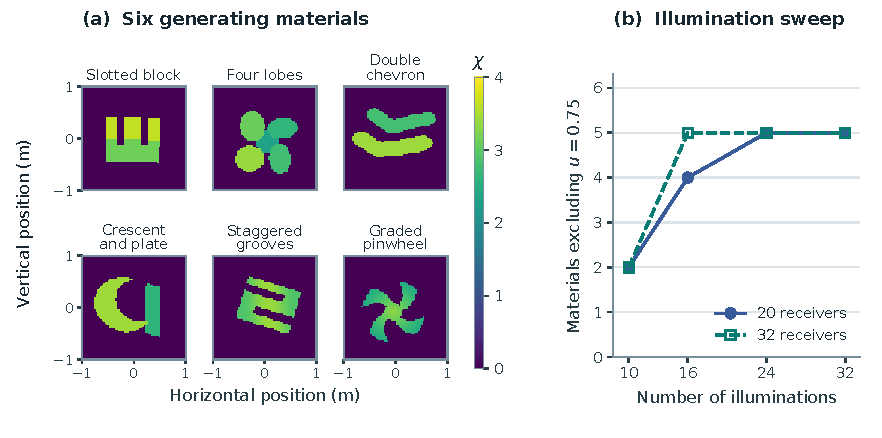
\includegraphics[width=.96\linewidth]{geometry.pdf}
\caption{The six independent dielectric distributions on a common contrast scale. At right, the number for which the measured data exclude a peak of 0.75, at equal total incident fluence and 2\% noise. Each point uses the same six objects.}
\label{fig:geometry}
\end{figure}

Half-ring reception leaves a substantial radiative component in the unmeasured current. On the native $96^2$ grid the leading numerical eigenvalue of $R_0$ is 4.805 for the half ring and 0.544 for the full ring, with $\|R\|_2\simeq5.095$ in the same units. For the denser receiver arrays of the compact annular and Austria tests, rigorous upper bounds on $\|R_0\|_2$ are respectively $7.56\,10^{-15}$ and $3.03\,10^{-10}$ in their own normalizations. At a cap of 0.5 and 2\% noise on the half ring, the tested real sector alone gives zero exclusions out of six. Adding optical balance gives six. At 10\% noise, adding quadrant balances to the global optical test increases the count from two to three. On the full ring the real sector already excludes 0.5 in all six cases at either noise level. These ablations fix the data within an aperture. In the comparison between apertures the illumination directions change as well.

At 2\% noise, ten incident fields and twenty full-ring receivers give a rigorous separation from tests with just one coherent combination. For Slotted block and Staggered grooves, the joint distances at cap 0.75 exceed 0.16069 and 0.11060, compared with radii 0.09097 and 0.08803. For each unit coherent input, a single current fits the receivers under both global balances. Under four regional balances and a uniform, physically necessary energy cap, a positive semidefinite lift also fits every coherent input exactly. Appendix~\ref{app:tech} gives the construction. With sixteen regions, particular coherent inputs do exclude the cap, at distances 0.18967 and 0.12452. The practical distinction depends on both the number of independently tested source directions and how much spatial variation the balances retain.

\subsection{Lossless media at increasing peak and electrical size}

On the 32-source, 32-receiver data at 2\%, one fixed, spatially constant profile excludes 0.78125 on five objects, 0.8125 on three, and 0.84375 on Crescent and plate alone, where $d/r>1.31$. These are improvements in resolution of the cap sweep using the rank bound. Several intervening or larger caps could not be settled by the selected Fourier floor. We show them as unresolved. At cap one the strongest previously evaluated scalar profile on these six data has $\nu=13$. In units of its scale $\mu=1.3535749382\,10^{-5}$, the negative and positive gaps exceed 0.03017 and 0.0019531. The source basis is 32-dimensional. Directly retaining the source eigenvalues gives at most $0.30106r$ on the six cases. Maximizing each ordered lower eigenvalue separately over the available profiles brings this to $0.30604r$ as a lower endpoint.

\begin{figure}[tbp]\centering
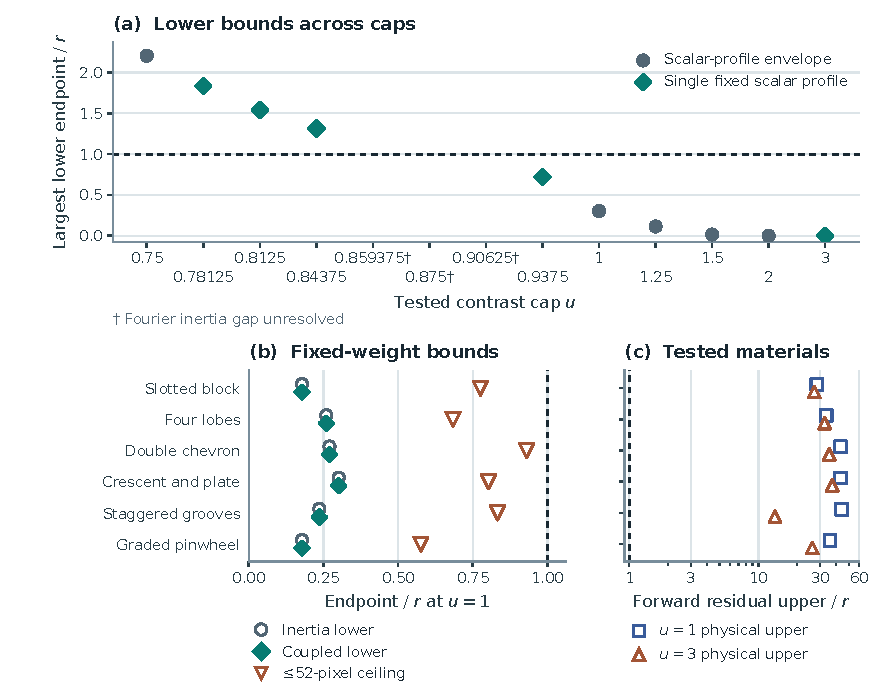
\includegraphics[width=\linewidth]{full-domain.pdf}
\caption{Lossless contrast tests on the full search square. Measured lower distances, upper limits on a family of local tests and residuals achieved by actual box-constrained materials answer three distinct questions. Missing spectral enclosures are indicated separately. The threshold line is the radius of the same data ball for all methods on one object.}
\label{fig:whole}
\end{figure}

We first attempted to recover source eigenvalues by local compensation on the same operator. The full positive spectrum was eliminated using the row Gram in Appendix~\ref{app:tech}. Rows were proposed by rank-revealing QR on negative-mode endpoint responses. For the 52-row calculation, the 104-by-104 endpoint Gram upper enclosure required an upward shift below $4.75\,10^{-9}$ in its normalized units. A center-aware semidefinite fit, including interval constraints on every selected material, gave $d/r>0.30104$ for Crescent and plate. The rank bound already gave $d/r>0.30105$. Failure of that particular selection did not settle whether other pixels could do better.

Applying Proposition~\ref{th:obstruction} to the \emph{entire} pixel pool gives a different conclusion. At an admissible material, the trace on the full negative space is below 0.98227 for any 29 separately weighted constitutive rows and below 1.98201 for any 59. Thus the former can compensate no negative direction and the latter at most one. This conclusion follows by sorting bounds for all 9,216 cells. Including the center with either sign of $M_Y$, Table~\ref{tab:scope} gives upper endpoints at 52 cells. At 59 cells the largest upper endpoint among the six is still below $0.97803r$. These counts refer to this grid, these state weights and nonnegative weights on individual constitutive rows. The computations also allowed a coupled positive semidefinite metric on each of three specific nested row sets of sizes 8, 26 and 52. The smallest eigenvalues of their signed row Grams exceeded 0.9790, 0.9471 and 0.8335 for suitable uniform test materials. None can uniformly compensate one negative direction, including after retaining additional positive modes explicitly in the local row calculation.

\begin{table}[tbp]\centering\small
\caption{Same native data and cap $u=1$. The first two columns are attained lower endpoints divided by $r$ at the same fixed current weights. The third is an upper endpoint on \emph{any} diagonal local compensation bound using at most 52 cells including signed center corrections. The fourth is the residual upper endpoint of an actual candidate material. The last two columns bound different mathematical quantities.}
\label{tab:scope}
\begin{tabular}{@{}lrrrr@{}}\toprule
Object & Rank & All-cell defect & 52-cell limit & Trial residual\\\midrule
Slotted block & .17833 & .17839 & .77551 & 28.330\\
Four lobes & .25949 & .25957 & .68392 & 33.363\\
Double chevron & .27019 & .27035 & .93030 & 43.231\\
Crescent and plate & .30105 & .30115 & .80274 & 43.154\\
Staggered grooves & .23632 & .23640 & .83274 & 44.094\\
Graded pinwheel & .17837 & .17850 & .57643 & 35.752\\\bottomrule
\end{tabular}
\end{table}

On larger selected sets of 208 and 416 cells the trace comparison gives $c\le3$ and $c\le4$, respectively. Even an ideal zero center charge would require $c\ge7,5,5,5,5,7$ in object order to reach the data radius. These last impossibility conclusions use $M_Y\succeq0$. Allowing all 9,216 cells still gives $c\le8$ for diagonal nonnegative frames at these weights. A second test retained two, four or eight weak positive current modes explicitly before bounding the remainder by a uniform Young inequality. Even after optimizing its scalar split, the number of compensated directions cannot exceed two, two or three, respectively, on this fixed split. A zero or nonnegative center charge would require at least five. Results for signed charges beyond the proved cardinality range and for freely varying frames remain open. At cap 1.25 another fixed profile has fifteen negative directions. Any 60 local rows have $c=0$, and up to 30 cannot yield an exclusion on any object even with a signed center.

We then used the full-box calculation \eqref{eq:full_def} with all cells. Choosing $\omega/\mu=10^{-3}$ and $\eta/\mu=2^{-20}$ preserves the index bound of thirteen and increases all six source lower endpoints slightly (Table~\ref{tab:scope}). The large local constitutive defects in the strongest illumination directions contribute little here because the first thirteen source eigenvalues are lost to interlacing. More aggressive weights spend additional negative directions and lose further source eigenvalues. This trade is present on the original grid and survives interval evaluation of the full stationary currents. In parallel, nonlinear box-constrained fits were initialized by coarse material updates, bounded Gauss--Newton, projected gradient and contrast-source inversion. Across eighteen object--cap combinations up to $u=3$ the best candidate in each tried combination was replayed by an independent full-grid state solve. At $u=3$ their smallest residual upper endpoint is $13.408r$. The lower sides of the individual fit residual intervals also exceed $r$. No search established physical feasibility under these caps. No lower-bound calculation at $u=1$ excluded them. A separately generated disk of peak 0.625 on the $96^2$ grid passes the $u=0.75$ physical control at $0.99995r$.

Changing the state weights offers a separate test. Divide the square into sixteen equal tiles and multiply the sector weight on the twelve outer tiles by 1.5 or 2.5, leaving the four central tiles and optical weight unchanged. All material pixels remain unknown. The exact full-state negative counts fall from thirteen to eleven and eight. The largest $d/r$ rises from 0.30105 to 0.31134 and 0.32376, respectively. For the second weight the projection onto the original thirteen modes counts only five negatives. Combining that count with the full source matrix gives spurious numerical threshold crossings on five objects. Even where the projected count agrees at the first weight, using its projected stationary field gives apparent ratios between 2.27 and 6.24 on all six. The full calculation puts every one below 0.312. Both errors result from truncating the current state before changing the quadratic. Reflection symmetry allows all four parity sectors of the actual operator to be checked without a material symmetry assumption (Appendix~\ref{app:tech}).

The same six unresolved observations do constrain which currents a successful reconstruction would have to contain. Setting the actual current component on the negative eigenspace to zero makes a cap-one fit impossible on \emph{all six} objects. The lower endpoints in \eqref{eq:required} for its Frobenius norm, in object order, are 15.75, 9.05, 14.42, 22.00, 19.76 and 7.65 in the unweighted discrete current coordinates. With zero such current the measured source forms alone would require residuals above $1.19r$ on every object. This rules out an exact truncation of that specific state subspace within the tested cap, even though the complete cap remains open. A legal cap-one candidate for Slotted block has negative current norm above 41.85 and misses the measured ball. Therefore any data-independent scalar upper norm valid over the whole box must allow at least that much current. The particular lower norms obtained here cannot be turned into full material exclusions by imposing a smaller scalar ceiling. The independent low-peak disk has negative current norm 18.39956 in its own error ball. A physical scatterer can drive these modes at modest contrast (Figure~\ref{fig:modes}).

\begin{figure}[tbp]\centering
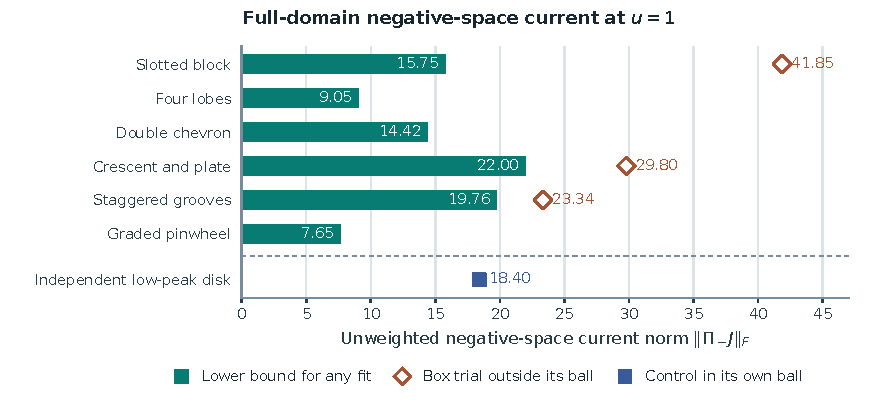
\includegraphics[width=\linewidth]{current-modes.pdf}
\caption{How much of the physical current must occupy the 13 negative modes at a contrast cap of one? Bars give lower bounds for any fit to the six observations. Open symbols mark full-wave currents of three box-admissible candidates outside their measured balls. The square marks a low-peak control which fits its own data. All amplitudes use the same total incident fluence and unweighted discrete current norm.}
\label{fig:modes}
\end{figure}

Compact media show why the domain matters. On a separate, electrically smaller $24^2$ annular problem with twelve illuminations and four negative modes, one unchanged profile excludes a peak of five on five of seven independent materials at 1\% noise, with ratios 5.12--10.77. One of the other two really does fit below cap five, with a peak of 4.28. On twenty-two additional $96^2$ lossless objects with 10\% noise the joint calculation excludes 0.5 on all twenty-two, whereas none clears 0.75. These transfers cover different independently generated materials. A native result on a compact search region cannot be used as a uniform bound for a larger one.

\subsection{What a specified loss or a calibrated instrument adds}

The dissipative comparison uses new full-wave observations for every $t\in\{0.01,0.05,0.2\}$. Two fresh distributions were generated in each of two domain widths. All pixels remained free in the inverse problem. Figure~\ref{fig:diss} compares bounds at fixed material law, using identical data and noise radius. On the $0.6\,\mathrm m$ square at $t=0.2,u=1$, the two receiver-ellipsoid lower endpoints are $1.17917r$ and $1.23174r$. For the first material $r=0.05609216459$. A single interval calculation over \emph{all} common nonnegative penalties and optimal coherent source projectors gives $d<0.99873r$. The same physical information thus suffices or fails to exclude a material class depending on how its source dependence is retained. Even a fixed right-singular basis of $Z_Y$, with separate scalar penalties, gives $d>1.14159r$ and $d>1.10601r$ for the two objects. Applying separate penalties in the original illumination basis gives only $0.57351r$ for the first object.

\begin{figure}[tbp]\centering
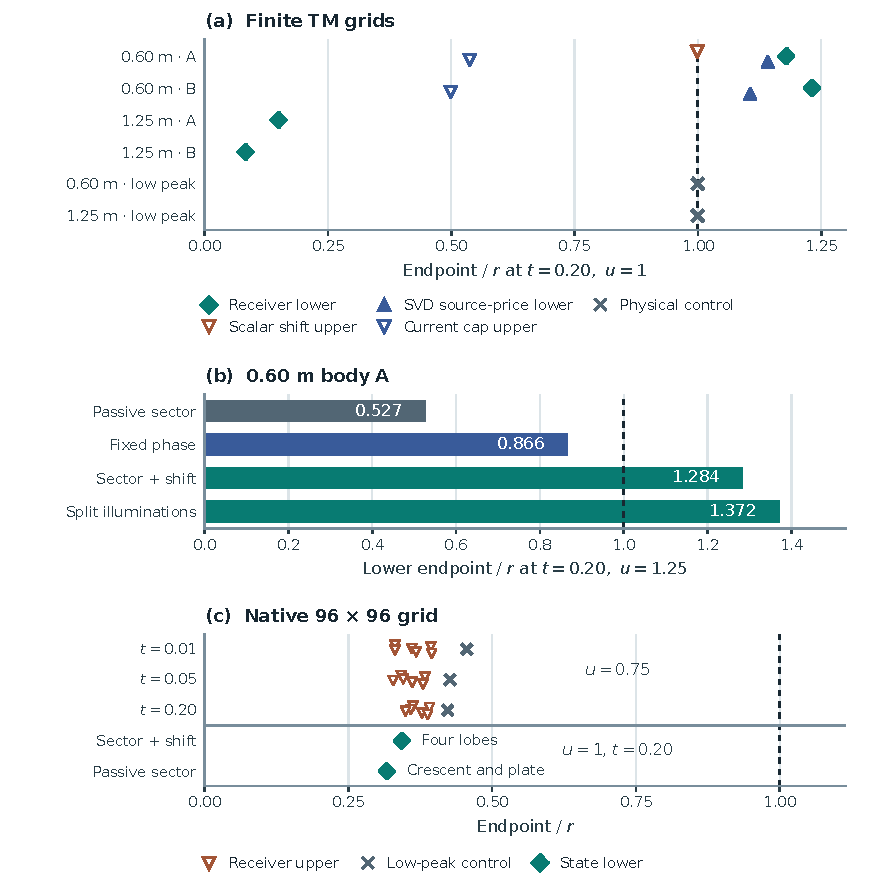
\includegraphics[width=\linewidth]{dissipation.pdf}
\caption{Bounds on the real contrast for specified loss tangents. Comparisons at the same loss tangent use the same complex data. Feasible points of a receiver ellipsoid upper-bound its distance, while only the verified low-peak material establishes a physical fit.}
\label{fig:diss}
\end{figure}

At the smaller loss tangent $t=0.05$ and cap $u=0.75$ the first object gives a wider separation. Subdivision of the complete common-penalty half-line gives a distance below $0.80975r$, while independent penalties in a fixed coherent basis give a lower bound above $1.01323r$. Direct projection raises this to $1.02003r$. On the second object the receiver distance is below $0.94901r$. At $t=0.2,u=1.25$ a whole-current dissipation shift \emph{combined with the sector} gives $d>1.28439r$ on the first object. The full receiver ellipsoid here has a distance below $0.66362r$. Using the same sector weights on a joint source block and independent receiver penalties on the orthogonal block raises the lower bound to $1.37213r$. After separately improving the sector weights, the matched whole-sector bound and the split give $1.51977r$ and $1.59135r$. These compare attained sector choices. At the higher cap 1.5 neither object is ruled out. For the first, the split reaches $0.61127r$ and the whole receiver ellipsoid alone gives more than $0.65218r$. For the second, the split reaches $0.72916r$, exceeding both the whole-sector result $0.59887r$ and the receiver distance upper endpoint $0.61437r$. The partitions were proposed using the measured source spectra and verified on the original matrices. The search scored all $2^{10}-2$ nonempty proper subsets in each of two data-derived coherent bases. An exhaustive subset search would grow exponentially with source count. At $u=1,t=0.2$ on the $1.25\,\mathrm m$ square, the two relaxed receiver distances are below $0.151r$ and $0.084r$. Finally, on the six $96^2$ shapes, even the tightest tested cap of 0.75 admits a receiver-ellipsoid point within $0.395r$ for each of the three loss tangents. Nesting proves that receiver projection alone cannot exclude any larger cap on those observed data. This statement concerns the exact outer sets. It does not produce a low-peak material.

For the finite examples one right-singular basis and its scalar solves cost 0.88 ms of CPU for the first object at $t=0.2,u=1$, after the common port Grams and bases had been formed. Direct iterative projection reached its 2,500-iteration limit after 0.319 s of CPU and supplied a valid dual direction. These figures exclude the shared setup and the separate interval evaluation and describe the computation of a proposal. On the larger array the corresponding median CPU times were 2.2 ms and 1.19 s. The six paired compact source-partition tests and their interval evaluations took 10.30 s wall time and 9.86 s CPU. An independent check of the positive spectral gaps added 0.54 s wall time and 0.52 s CPU. Detailed costs, including unsuccessful fits, are given in Appendix~\ref{app:tech}.

Two laboratory datasets set a separate limit on interpreting any positive lower bound. With measured total minus incident fields for the three Fresnel cylinders at 4, 6 and 8 GHz, none of the nine views clears the held-out empty-scene scale at a cap of 0.5 \cite{fresnel}. At cap 0.25 the twin target at 4 GHz leaves $6.98\%$ of the receiver norm for additional discrepancy after budgeting additive error and gain. In Manitoba four physical objects at seven frequencies are compared under four receiving calibrations \cite{manitoba}. Subtracting the largest displacement among these calibrations leaves a positive allowance in 20, 5, 3 and 1 of the 28 views at passive disk caps 0.25, 0.5, 0.75 and 1. The large nylon cylinder at 3 GHz leaves $4.018\%$ at cap one. These are explicitly conditional margins. Neither laboratory supplies a uniform bound on loaded-scene error for every hypothetical medium.

The same distinction matters when changing the object of the test. A sixteen-region localization test with unconstrained surroundings gave zero positive local bounds in 112 regional cases. A principal block in the exterior alone supplied enough negative directions to exhaust all available illuminations for the specified weight range. In a joint 400/500 MHz half-aperture comparison, three of six nominal low-cap decisions from separate frequencies became zero of six after adding the measured coarse-grid discrepancies. Conversely, enlarging a contrast range after ruling out a low peak on a compact patch reduced held-out complex-field error from 27.50\% to 1.32--2.52\%, while final relative material error rose from 0.462 to 0.721--0.943. An ordinary discrepancy stopping rule recovered much the same final fit. A full-class exclusion is a useful statement about the data even in a case where it gives no advantage in image accuracy.
\FloatBarrier


\section{Discussion and conclusion}\label{sec:discussion}

A lower bound on peak contrast can be useful at a stage where estimating its location or its actual value remains difficult. To rule out a real cap, the receiver data must leave a positive source spectrum after accounting for the admissible hidden currents. On a limited aperture the optical balance can suppress radiating currents missed by the array. With denser reception the remaining current modes may radiate weakly, and sharing their dimension across illuminations becomes more useful. Adding illuminations eventually repeats angular information. None of these phenomena can be read from the clean field norm alone.

The central limitation of a sparse local correction has a physical interpretation. A chosen cell can always sustain some accompanying positive current. For a correction to restrict a negative mode throughout an unknown dielectric, the same row weights must charge that mode more than they charge every possible positive current. The operator often allows many weak directions to avoid those cells. Bounding this possibility over all choices of the cells gives a stronger diagnosis than reporting a failed semidefinite solve. The diagnosis is conditional on a particular quadratic form and a specified representation of the local rows. It still permits tighter joint constraints, different physical weights and material laws. Even zero negative inertia does not convexify the actual set of physical currents. For $G=\mathrm i$, $S=B=1$ and $x\in[0,1]$, the midpoint between $J(0)$ and $J(1)$ would require $x=2/5+\mathrm i/5$.

When the dissipative coefficient is bounded away from zero, an independent restriction survives projection onto the ports. On a compact object, two loss angles give strict separations for the same dissipative information. A fixed coherent basis captures much of the gain. Assigning different orthogonal source blocks to the sector and to dissipation further sharpens an attained distance bound, with no change to the highest excluded contrast in those trials. The larger examples delimit that result. Even an exact computation of distance to the dissipative ellipsoid cannot distinguish the measured data from the relaxed cap there. A smaller numerical step or an improved ellipsoid solver cannot remove the physical information discarded by that projection. The fixed-loss-angle examples also should not be used to strengthen a lossless contrast conclusion.

For laboratory use the most consequential missing quantity is a reliable bound on loaded-scene model discrepancy. An independently measured receiver drift constrains part of this error. It cannot by itself control imperfect incident fields in the loaded chamber, three-dimensional coupling or uncertain target properties. At fixed frequency the continuum mode asymptotic explains why contrast makes the current restriction harder. Transfer of a computed finite-grid distance to an unknown continuum coefficient would additionally require a uniform forward approximation bound on its whole admissible class. In inversion an observation may therefore rule out an entire material hypothesis while the remaining image, its peak location and an optimizer's route to it remain separate questions.

\appendix
\section{Proof details and reliable numerical endpoints}\label{app:tech}

\subsection*{Eliminating the positive current at fixed rows}

For the row relation in \eqref{eq:rows}, singular values of the restricted positive Green operator can be small. A padded inverse with an arbitrary ridge would change the optimization. For a given material tuple $x$ set $Z=D_x-T_x C$. If $Z$ lies in the range of the positive-row map $F_+$, its minimum positive Gram is exactly $Z^*(F_+F_+^*)^\dagger Z$. Otherwise the local tuple is impossible. For a necessary relaxation one may drop this range condition and take an outward upper envelope of $F_+F_+^*$, adding the appropriate range treatment or a positive floor. A trace, directional ellipsoid or eigenvalue bound on $C^*C$ may be intersected with these restrictions provided it holds for the full material hypothesis. A bound derived assuming $\|SJ-Y\|\le r$ can establish inconsistency of that ball. It cannot be inserted without qualification into a lower bound on $\delta(u;Y)$ outside the ball.

Two short checks delimit the rank argument. If $K$ is singular and $\Pi_{\ker K}L=0$, use $K^\dagger L$ in \eqref{eq:center}. The null coordinates contribute zero to completion. Subsequent local row equations must retain these free variables. If the range condition fails, the linear current term along the null directions cannot be discarded. Compression to the source directions annihilating $\Pi_{\ker K}L$ gives a lower bound on that part of the residual. For the main numerical comparisons an open spectral gap is checked on both sides instead.

A uniform receiver-exact fit for each separate coherent input need not hold jointly. For a collection of balances in spatial regions $b$, let $J_a=C_0a$ with $SC_0=Y$ and $w_j\in\ker S$. For any $P_j\succeq0$ use $\sum_j(a^*P_ja)w_jw_j^*$ as the current covariance for input $a$. The moment data fit exactly. With $D_b$ the indicator of a region, its sector and optical values receive the source-matrix increments
\[
 \sum_j[\|D_bw_j\|^2-u\Re(w_j^*D_bGw_j)]P_j,\qquad
 \sum_j\Im(w_j^*D_bGw_j)P_j .
\]
Satisfying the resulting matrix inequality and equality in each region constructs a feasible lifted current for every unit $a$ at once. Its energy is bounded by the largest eigenvalue of $C_0^*C_0+\sum_j\|w_j\|^2P_j$. In the two four-region examples of section~\ref{sec:experiments}, eight invisible directions suffice. The respective energy bounds are 8,500 and 7,000. A physical response in the same material box has energy above 8,886.62, so a scalar cap valid uniformly for the box and all unit inputs cannot eliminate those fits. Output-dependent caps on each complete error ball, $4.983\,10^6$ and $1.035\,10^6$, also admit them. These are statements about coherent relaxations. There is no assumption of strong duality for an arbitrary problem with several quadratic constraints \cite{beck}.

For the global sector and optical balances alone, a stronger constructive argument is possible. Write $q_r(j),q_o(j)$ for a unit input and its current balances. Suppose one receiver-null vector $w$ has $\rho=w^*Rw>0$ and $w^*(I-u\Herm G+t_0R)w<0$. Suppose $x=C_0a$ has $q_o(x)<0$ and $q_r(x)+t_0q_o(x)<0$ for all unit $a$. Choose $|\beta|^2=-q_o(x)/\rho$ and choose a phase of $\beta$ cancelling the optical cross term. Of the two opposite such phases, one has nonpositive sector cross term. Thus $x+\beta w$ satisfies both global balances and keeps the receiver fit. A covariance $\epsilon I+c_\epsilon ww^*$, with $c_\epsilon=(-q_o(x)-\epsilon\tr R)/\rho$, gives a relative Slater point for the lifted global problem for small $\epsilon>0$, since the sector remains strict. The coherent dual optimum is then zero \cite{boyd}. This is a data- and operator-dependent sufficient construction.

Conversely, a joint moment relaxation averages over currents. Each sample can spend a different negative source direction, so the rank of the average need not be bounded by $\nu$. In a five-cell reciprocal algebraic control with $R=I/20\succ0$, a four-point current distribution satisfies the averaged balances and has zero receiver variance, while a single negative direction leaves the positive squared-distance bound $2317/2400$. The physical squared distance is $800/401$. Conversely a positive source matrix multiplier can strengthen the scalar-current construction. In a two-cell zero-propagation control its lower bound is $88/47$, while every scalar-weight comparison in that example is at most $373/200$. These exact controls are given with their matrices in the numerical supplement. Positive-semidefinite lifting and pointwise interlacing exploit different restrictions.

\subsection*{A center term that changes an exclusion}

For a passive reciprocal algebraic example take $u=\mu=1$, $\lambda=0$ and
\[
 G=\begin{pmatrix}2+\mathrm i/2&1/4\\1/4&\mathrm i/2\end{pmatrix},\quad
 S^*S=\begin{pmatrix}1/2&1/4\\1/4&1/2\end{pmatrix},\quad
 B=\begin{pmatrix}-3/4-2\mathrm i\\5/4+9\mathrm i/2\end{pmatrix}.
\]
Choose $Y=S(1,-3+6\mathrm i)^\top$, generated by $X=2I$. The hypothesis is the entire real square $[0,1]^2$. Then $K=\diag(-1/2,3/2)$, $J_0=(5/4-\mathrm i,-5/12+7\mathrm i/2)^\top$, $(E_0)_1=103/48-5\mathrm i/2$, and $H=199/48$. There is one source and one negative direction. At cell one, $\omega_1=24$ gives $\omega_1|f_1(x)|^2=x^2$. For $c=1$ and $M_Y=3/2$ the first leading minor of \eqref{eq:comp} is $204x^2-192x+47\ge31/17$. Its determinant is $(4367x^2-3768x+864)/96>0$, since its discriminant in the numerator is negative. Therefore $\delta^2\ge127/48$ or $35.0802\%$ of the signal norm in distance. The rank bound is zero at these fixed weights. Uniformly bounding the norm of the center separately from the negative-row gain gives a subtraction exceeding 73 and again gives zero. This passive algebraic example does not use an open-domain Helmholtz geometry.

\subsection*{Whole-current and projected dissipation}

Split the negative term in \eqref{eq:started} as $\|W_c(J-J_0)\|^2+\|W_f(J-J_0)\|^2$, interpreted as source Grams. Let $W_f$ have $m$ rows. For $\Gamma=W_cM^{-1}W_c^*$ and $Z_0=W_c(J_c-J_0)$, completion at $\tau>\|\Gamma\|_2$ gives, for every $J$,
\begin{multline*}
 \tau(J-J_c)^*M(J-J_c)
 -(J-J_0)^*W_c^*W_c(J-J_0)\\
 \succeq-\tau Z_0^*(\tau I-\Gamma)^{-1}Z_0 .
\end{multline*}
Subtract $\tau C_B$ and add to the original quadratic. The fully shifted form dominates $H-\mathcal B_\tau-(J-J_0)^*W_f^*W_f(J-J_0)$ for every free $J$. Its free residual epigraph, with $\mathsf D\succeq0$, therefore has minimum trace at least $\Tail_m(H-\mathcal B_\tau)$. For nonsingular shifted state matrix, rank interlacing attains the free minimum by completion of squares. Thus feeding the same scalar into the whole dissipation constraint weakly dominates the partial matrix cap at that scalar. The rank cap can be cheaper to evaluate when projected quantities are already available. A singular transition is handled by a nondegenerate neighboring weight and a limit of lower bounds. Source-dependent multipliers in \eqref{eq:prices} escape this comparison.

For the strict comparison with all common dissipative prices, let $B_\tau=Z_Y^*(R_S+\tau I)^{-1}Z_Y-C_B$. It decreases with $\tau$. Hence for $0\le a\le\tau\le b$, $\tr[H(\tau)]_+\le b\,\tr[B_a]_+$. We interval-evaluated this expression on 101 intervals through an endpoint greater than $6.70676$ for $t=0.2$, $u=1$. At the actual right endpoint $B_\tau\preceq0$ and remains so. For $t=0.05$, $u=0.75$, the same calculation uses 92 intervals to $3.73262$, beyond which the positive trace vanishes. This proves the upper bound over a continuum of prices used in section~\ref{sec:experiments}. The lower bounds in coherent bases use intervals about the exact unitary polar factor of the stored basis. The receiver primal upper endpoints use explicit contractions. These computations bound an optimization in receiver space. A feasible receiver point can have no material preimage.

\subsection*{Native grid arithmetic, work and continuum scope}

The discrete convolution is a compression $G=V^*\diag(g)V$ of a $192^2$ padded Fourier multiplier by an isometry $V$. For scalar weights the Hermitian state form is the compression of a real symbol plus $S^*S/\mu$. Bounding the omitted symbol from below by a scalar floor leaves a positive diagonal and signed finite-rank Fourier updates. A small signed Gram congruence bounds the state negative count from above. An interval negative subspace of the full native operator gives the matching lower count. A failure of a floor to settle a gap is retained as unresolved. For quadrant-reflection invariant weights a separate check decomposes the reflection-averaged Hermitian operator into four parity blocks, each of size 2,304. In each block a low-rank update $WW^*$ raises the trial negative modes above zero. A Cholesky residual, including bounds for assembling the matrix, proves a strictly positive floor for the updated block. Interlacing bounds the number below that floor by $\rank W$. The norm error of reflection averaging, including the receiver Gram and stored kernel, is subtracted before combining the blocks. Independent negative Rayleigh subspaces on the original grid supply the reverse count. Symmetry is used only for the state weights and array. The material still varies independently at every pixel. For the all-cell test, $X=(u/2)I+\Delta$ with $\|\Delta\|\le u/2$ yields
\[
 \|(I-XG)z\|^2\le
 2\|(I-uG/2)z\|^2+\tfrac{u^2}{2}\|Gz\|^2 .
\]
The compressed Fourier norm is bounded by the corresponding uncompressed norm. The same calculation now applies to a symbol with the additional subtraction $\omega[2|1-ug/2|^2+u^2|g|^2/2]$. At the selected weight 441 retained Fourier modes and the receiver Gram suffice to put the full-box negative count at most thirteen. Trial residuals are evaluated by ball arithmetic on the original grid, including the cross term in \eqref{eq:trial}.

For any row block $A$ the positive Gram is $A K_+^\dagger A^*$. On the positive space take a block solution trial $Z_+$ and residual $\Delta=\Pi_+ A^*-K Z_+$. With $g_+>0$ a verified positive spectral gap,
\[
 A K_+^\dagger A^*\preceq A Z_+ + Z_+^* A^* - Z_+^* K Z_+
                              +g_+^{-1}\Delta^*\Delta .
\]
This follows by completing a square with exact remainder $\Delta^*K_+^\dagger\Delta$. Projection errors, repeated eigenvector clusters, the stationary residual and both centers must be enclosed. We reorthogonalized the low eigenspace and checked its leakage into the opposite space. The upper leakage at cap one was $2.2\,10^{-11}$. Endpoint stacks at $x=0,u$ give a uniform sufficient frame using convexity of the squared norm of an affine row. For the center-dependent block, candidate univariate summands were checked on each whole interval by coefficient comparison with $[I;xI]^*P[I;xI]+x(u-x)Q$ for positive matrices $P,Q$. Inexact polynomial coefficients, trial positivity and the center terms enter one-sided error allowances. Small semidefinite proposals and iterative eigenpairs are not themselves error enclosures. Final checks use real and complex ball arithmetic \cite{arb}.

The optical and stationary operators are shared by all observations with the same array, cap and weights. The main cap-one center and inertia run took 121 s wall time. Correcting the projected basis took another 21 s, and the full one-sided 104-row Gram and sparse bounds took 87 s. A separate proof for the dense supports took 12 s after 19 s of proposal time. The independent whole-domain source calculation took 159 s including verification. For the two edge weights, checking all four reflection subspaces and the six source matrices took 311 s wall time and 298 s CPU in total. Across all eighteen physical endpoint checks the inversion proposals used 426 native full-wave evaluations and 591,441 floating-point FFT columns. The final interval evaluations used 576 additional columns and 146 CPU seconds. These are measured costs for different outputs. Counting only a final source-space diagonalization would hide most of the work.

For clarity about the continuum statement \eqref{eq:weyl}, localize to a larger bounded region and replace the singular part of $H_G$ there by the positive model $k^2(1-\Delta_{\R^2})^{-1}$. Its difference has lower order than $-2$, since the outgoing resolvent has the same high-frequency principal symbol and the remainder away from the diagonal is smooth. The signed eigenvalue counting function of this localized remainder is $o(\varepsilon^{-1})$ \cite{ponge}. Compression cannot increase its singular values. For the leading operator $A\ge0$, compression to $\Omega$ has the same nonzero spectrum as $A^{1/2}{\bf1}_\Omega A^{1/2}$. When $|\partial\Omega|=0$, smooth squared cutoffs below and above the indicator sandwich this in the operator order, with integrals tending to $|\Omega|$. This includes a square. The compact-support negative-order Weyl law gives $k^2\int\varphi^2/(4\pi\varepsilon)$ for each such cutoff. The variational counting inequalities with a fractional threshold for the lower-order part give the same leading constant after that fraction tends to zero. Finally decompose $C$ into a finite-rank part and a remainder of norm below any $\epsilon>0$. Interlacing places the count between those of $H_G$ at thresholds $(1\pm\epsilon)/u$, up to a fixed finite number of modes. Taking $u\to\infty$ first proves \eqref{eq:weyl}. This derivation supplies no uniform discretization error or frequency-dependent remainder estimate.

If $\|Y-Y_{\rm model}\|_F$ includes additive uncertainty $a$, gain error $\eta_g<1$, and a separately justified loaded-scene discrepancy $b$, these enter the distance comparison in receiver units. For diagonal gains of operator norm error at most $\eta_g$, a conservative budget from a measured field norm is $(a+b+\eta_g\|Y\|_F)/(1-\eta_g)$ when $a,b$ are additive errors in the observed coordinates. An empirical empty-scene discrepancy supplies a calibration scale. A deterministic claim about a loaded target requires a bound appropriate to that target and the admitted physical models.


\section*{Data availability}
The synthetic data, discrete operators, plotting sources and numerical enclosures accompany the article. References \cite{fresnel,manitoba} describe the measured data. Public project identifiers are provided separately for double-anonymous review.
\section*{Acknowledgments}
\textit{Use of generative AI.} OpenAI Codex (GPT-6.2 Astra and Sol) assisted with the analysis, software, experiments and writing. Google Gemini Neon provided independent pre-submission mathematical and experimental critiques. Exact algebraic controls, independent forward computations and outward-rounded spectral calculations were used to check the reported numerical results. The research supplement documents these checks and their limits.
\begin{thebibliography}{99}
\setlength{\itemsep}{2pt plus 0.5pt minus 0.2pt}
\bibitem{chen} Chen X 2010 Subspace-based optimization method for solving inverse-scattering problems \emph{IEEE Trans. Geosci. Remote Sens.} \href{https://doi.org/10.1109/TGRS.2009.2025122}{\textbf{48} 42--49}
\bibitem{zhong} Zhong Y and Chen X 2009 Twofold subspace-based optimization method for solving inverse scattering problems \emph{Inverse Problems} \href{https://doi.org/10.1088/0266-5611/25/8/085003}{\textbf{25} 085003}
\bibitem{ffttsom} Zhong Y and Chen X 2011 An FFT twofold subspace-based optimization method for solving electromagnetic inverse scattering problems \emph{IEEE Trans. Antennas Propag.} \href{https://doi.org/10.1109/TAP.2010.2103027}{\textbf{59} 914--927}
\bibitem{angeris19} Angeris G, Vu\v{c}kovi\'{c} J and Boyd S P 2019 Computational bounds for photonic design \emph{ACS Photonics} \href{https://doi.org/10.1021/acsphotonics.9b00154}{\textbf{6} 1232--1239}
\bibitem{trivedi} Trivedi R, Angeris G, Su L, Boyd S, Fan S and Vu\v{c}kovi\'{c} J 2020 Bounds for scattering from absorptionless electromagnetic structures \emph{Phys. Rev. Applied} \href{https://doi.org/10.1103/PhysRevApplied.14.014025}{\textbf{14} 014025}
\bibitem{angeris} Angeris G, Vu\v{c}kovi\'{c} J and Boyd S 2021 Heuristic methods and performance bounds for photonic design \emph{Opt. Express} \href{https://doi.org/10.1364/OE.415052}{\textbf{29} 2827--2854}
\bibitem{moleskyglobal} Molesky S, Chao P, Jin W and Rodriguez A W 2020 Global $\mathbb{T}$ operator bounds on electromagnetic scattering: upper bounds on far-field cross sections \emph{Phys. Rev. Research} \href{https://doi.org/10.1103/PhysRevResearch.2.033172}{\textbf{2} 033172}
\bibitem{moleskylocal} Molesky S, Chao P and Rodriguez A W 2020 Hierarchical mean-field $\mathbb{T}$ operator bounds on electromagnetic scattering: upper bounds on near-field radiative Purcell enhancement \emph{Phys. Rev. Research} \href{https://doi.org/10.1103/PhysRevResearch.2.043398}{\textbf{2} 043398}
\bibitem{kuang} Kuang Z and Miller O D 2020 Computational bounds to light--matter interactions via local conservation laws \emph{Phys. Rev. Lett.} \href{https://doi.org/10.1103/PhysRevLett.125.263607}{\textbf{125} 263607}
\bibitem{shim} Shim H, Kuang Z, Lin Z and Miller O D 2024 Fundamental limits to multi-functional and tunable nanophotonic response \emph{Nanophotonics} \href{https://doi.org/10.1515/nanoph-2023-0630}{\textbf{13} 2107--2116}
\bibitem{tian} Tian Y 2013 Closed-form formulas for calculating the extremal ranks and inertias of a quadratic matrix-valued function and their applications \href{https://arxiv.org/abs/1301.2567v1}{arXiv:1301.2567v1}, Corollary~4.5, equation~(4.38)
\bibitem{griesmaier_harrach}
Griesmaier R and Harrach B 2018 Monotonicity in inverse medium scattering on unbounded domains \emph{SIAM J. Appl. Math.} \href{https://doi.org/10.1137/18M1171679}{\textbf{78} 2533--57}
\bibitem{griesmaier_harrach_erratum}
Griesmaier R and Harrach B 2021 Erratum: monotonicity in inverse medium scattering on unbounded domains \emph{SIAM J. Appl. Math.} \href{https://doi.org/10.1137/21M1399221}{\textbf{81} 1332--37}
\bibitem{albicker} Albicker A and Griesmaier R 2023 Monotonicity in inverse scattering for Maxwell's equations \emph{Inverse Probl. Imaging} \href{https://doi.org/10.3934/ipi.2022032}{\textbf{17} 68--105}
\bibitem{bucci87} Bucci O M and Franceschetti G 1987 On the spatial bandwidth of scattered fields \emph{IEEE Trans. Antennas Propag.} \href{https://doi.org/10.1109/TAP.1987.1144024}{\textbf{35} 1445--1455}
\bibitem{bucci89} Bucci O M and Franceschetti G 1989 On the degrees of freedom of scattered fields \emph{IEEE Trans. Antennas Propag.} \href{https://doi.org/10.1109/8.29386}{\textbf{37} 918--926}
\bibitem{colton} Colton D and Kress R 2019 \emph{Inverse Acoustic and Electromagnetic Scattering Theory} 4th edn (Cham: Springer) \href{https://doi.org/10.1007/978-3-030-30351-8}{doi:10.1007/978-3-030-30351-8}
\bibitem{chenbook} Chen X 2018 \emph{Computational Methods for Electromagnetic Inverse Scattering} (Singapore: Wiley) \href{https://doi.org/10.1002/9781119311997}{doi:10.1002/9781119311997}
\bibitem{richmond} Richmond J H 1965 Scattering by a dielectric cylinder of arbitrary cross section shape \emph{IEEE Trans. Antennas Propag.} \href{https://doi.org/10.1109/TAP.1965.1138427}{\textbf{13} 334--341}
\bibitem{boyd} Boyd S and Vandenberghe L 2004 \emph{Convex Optimization} (Cambridge: Cambridge University Press) \href{https://doi.org/10.1017/CBO9780511804441}{doi:10.1017/CBO9780511804441}
\bibitem{beck} Beck A and Eldar Y C 2006 Strong duality in nonconvex quadratic optimization with two quadratic constraints \emph{SIAM J. Optim.} \href{https://doi.org/10.1137/050644471}{\textbf{17} 844--860}
\bibitem{manitoba} Gilmore C, Zakaria A, Mojabi P, Ostadrahimi M, Pistorius S and Lo Vetri J 2011 The University of Manitoba microwave imaging repository: a two-dimensional microwave scattering database for testing inversion and calibration algorithms \emph{IEEE Antennas Propag. Mag.} \href{https://doi.org/10.1109/MAP.2011.6138442}{\textbf{53} 126--133}
\bibitem{fresnel} Geffrin J-M, Sabouroux P and Eyraud C 2005 Free space experimental scattering database continuation: experimental set-up and measurement precision \emph{Inverse Problems} \href{https://doi.org/10.1088/0266-5611/21/6/S09}{\textbf{21} S117--S130}
\bibitem{everett96}
Everett M E 1996 Homotopy, polynomial equations, gross boundary data, and small Helmholtz systems \emph{J. Comput. Phys.} \href{https://doi.org/10.1006/jcph.1996.0070}{\textbf{124} 431--41}
\bibitem{vasco}
Vasco D W 2000 An algebraic formulation of geophysical inverse problems \emph{Geophys. J. Int.} \href{https://doi.org/10.1046/j.1365-246x.2000.00188.x}{\textbf{142} 970--90}
\bibitem{sivia}
Jaulin L and Walter E 1993 Set inversion via interval analysis for nonlinear bounded-error estimation \emph{Automatica} \href{https://doi.org/10.1016/0005-1098(93)90106-4}{\textbf{29} 1053--64}
\bibitem{chai}
Chai A, Moscoso M and Papanicolaou G 2014 Imaging strong localized scatterers with sparsity promoting optimization \emph{SIAM J. Imaging Sci.} \href{https://doi.org/10.1137/130943200}{\textbf{7} 1358--87}
\bibitem{levinson}
Levinson H W and Markel V A 2016 Solution of the nonlinear inverse scattering problem by \(T\)-matrix completion. I. Theory \emph{Phys. Rev. E} \href{https://doi.org/10.1103/PhysRevE.94.043317}{\textbf{94} 043317}
\bibitem{alberti19}
Alberti G S and Santacesaria M 2019 Calder\'on's inverse problem with a finite number of measurements \emph{Forum Math. Sigma} \href{https://doi.org/10.1017/fms.2019.31}{\textbf{7} e35}
\bibitem{alberti21}
Alberti G S and Santacesaria M 2022 Infinite-dimensional inverse problems with finite measurements \emph{Arch. Ration. Mech. Anal.} \href{https://doi.org/10.1007/s00205-021-01718-4}{\textbf{243} 1--31}
\bibitem{csi} van den Berg P M and Kleinman R E 1997 A contrast source inversion method \emph{Inverse Problems} \href{https://doi.org/10.1088/0266-5611/13/6/013}{\textbf{13} 1607--1620}
\bibitem{nie} Zhong Y, Lambert M, Lesselier D and Chen X 2016 A new integral equation method to solve highly nonlinear inverse scattering problems \emph{IEEE Trans. Antennas Propag.} \href{https://doi.org/10.1109/TAP.2016.2535492}{\textbf{64} 1788--1799}
\bibitem{cie} Zhong Y and Xu K 2019 Contraction integral equation for three-dimensional electromagnetic inverse scattering problems \emph{J. Imaging} \href{https://doi.org/10.3390/jimaging5020027}{\textbf{5} 27}
\bibitem{arb} Johansson F 2017 Arb: efficient arbitrary-precision midpoint-radius interval arithmetic \emph{IEEE Trans. Comput.} \href{https://doi.org/10.1109/TC.2017.2690633}{\textbf{66} 1281--1292}
\bibitem{fan} Fan K 1949 On a theorem of Weyl concerning eigenvalues of linear transformations I \emph{Proc. Natl Acad. Sci. USA} \href{https://doi.org/10.1073/pnas.35.11.652}{\textbf{35} 652--655}
\bibitem{douglas} Douglas R G 1966 On majorization, factorization, and range inclusion of operators on Hilbert space \emph{Proc. Amer. Math. Soc.} \href{https://doi.org/10.1090/S0002-9939-1966-0203464-1}{\textbf{17} 413--415}
\bibitem{miller} Miller O D, Polimeridis A G, Reid M T H, Hsu C W, DeLacy B G, Joannopoulos J D, Solja\v{c}i\'{c} M and Johnson S G 2016 Fundamental limits to optical response in absorptive systems \emph{Opt. Express} \href{https://doi.org/10.1364/OE.24.003329}{\textbf{24} 3329--3364}
\bibitem{ponge} Ponge R 2023 Connes\textquoteright{} integration and Weyl\textquoteright{}s laws \emph{J. Noncommut. Geom.} \href{https://doi.org/10.4171/JNCG/509}{\textbf{17} 719--767}
\end{thebibliography}

\end{document}

